%
% Report -- Verilog-A Logarithmic Amplifier Macromodel
%
% Copyright (C) 2008 Mike Brinson <mbrin72043@yahoo.co.uk>
%
% Permission is granted to copy, distribute and/or modify this document
% under the terms of the GNU Free Documentation License, Version 1.1
% or any later version published by the Free Software Foundation.
%

% redefine subfigure caption
\renewcommand{\thesubfigure}{\thefigure(\alph{subfigure})}
\makeatletter
  \renewcommand{\@thesubfigure}{\thesubfigure:\space}
  \renewcommand{\p@subfigure}{}
\makeatother

% redefine subtable caption
\renewcommand{\thesubtable}{\thetable(\alph{subtable})}
\makeatletter
  \renewcommand{\@thesubtable}{\thesubtable:\space}
  \renewcommand{\p@subtable}{}
\makeatother

\tutsection{Introduction}

The development of simulation component and device models in many ways
reflects how circuit simulator functionality has improved with
increasing personal computer computational power. Early circuit
simulators were often restricted to the DC, AC and transient analysis
domains.  Similarly, in the early days of circuit simulation, the
available types of component and device models were extremely limited,
often being confined to the fundamental passive components, simple
voltage and current sources and the basic semiconductor devices.
Adding new models to a circuit simulator was, in most instances, a
complex task. Today this picture is changing. Modern circuit
simulators, like Qucs, are equipped with an ever widening selection of
simulation tools plus increasingly sophisticated modelling tools. The
later allows easy construction of subcircuit models, linear and
non-linear macromodels, equation defined device models, and Verliog-A
compact device models.  This report describes how a compact macromodel
of a logarithmic amplifier can be constructed from a model description
written in the Verilog-A hardware description language, compiled to
C++ code using the ADMS compiler plus Qucs XML interface, and linked
to the main body of Qucs C++ code\footnote{A detailed description of
the procedure for the compilation of Verilog-A models with ADMS and
linking of the resulting C++ code to Qucs can be found in the Qucs
publication : ``Qucs Description: Verilog-AMS interface'', by Stefan
Jahn, H\'{e}l\`{e}ne Parruitte, located at
\url{http://qucs.sourceforge.net/docs.html}. }. The logarithmic
amplifier model demonstrates an approach to Qucs modelling which
allows high-level functional models of integrated circuits to be added
to the existing range of Qucs component and device models.

\tutsection{The ideal logarithmic amplifier}

The operation of an ideal logarithmic amplifier\footnote{A very good
introduction to the theory of logarithmc amplifiers is given in Sergio
Franco, Design with Operational amplifiers and Analog Integrated
Circuits, McGraw-Hill Book Company, ISBN 0-07-021799-8.} is defined by
the function given in equation \eqref{eq:vout}.
\begin{equation}
\label{eq:vout}
V_{out}(ideal)=K_{v}\cdot log\left( \dfrac{I_{i}}{I_{r}}\right)
\end{equation}

The device accepts two input currents ($I_{i}$ and $I_{r}$) and
outputs voltage $V_{out}(ideal)$ which is proportional to the base ten
logarithm of the current ratio $I_{i}/I_{r}$, where the constant of
proportionality is $K_{v}$ volts per decade.  In equation
(\arabic{equation}) current $I_{r}$ is called the reference current
and current $I_{i}$ represents the amplifier input signal. The primary
purpose of a logarithmic amplifier is not to amplify input signals but
to compress a wide dynamic range input signal to give as output it's
logarithmic equivalent. In some respects the name logarithmic
amplifier is misleading and it would be better to consider the
amplifier as a measurement device rather than an amplifier.  For the
ideal logarithmic amplifier when $I_{i}=I_{r}$, the output voltage
$V_{out}(ideal) \Rightarrow 0$. In a practical logarithmic amplifier
the current input terminals are effectively at virtual ground
potential which allows the amplifier input signals to be derived from
input voltages divided by scaling resistors of identical value. In
this case $I_{r}=V_{r}/R$ and $I_{i}=V_{i}/R$, where $V_{r}$ and
$V_{i}$ are the input signal voltages respectively, and $R$ is the
scaling resistance.  Transforming from current inputs to voltage
inputs gives equation \eqref{eq:vout2}.
\begin{equation}
\label{eq:vout2}
V_{out}(ideal)=K_{v}\cdot log\left( \dfrac{V_{i}}{V_{r}}\right)
\end{equation}

To prevent the argument of the logarithmic amplifier from becoming
negative the input signal $I_{i}$ must always have the same polarity
as reference signal $I_{r}$. The amplitude of the signal at terminal
$I$ must also be the same or greater than the signal at terminal
$R$. This implies that logarithmic amplifiers are unipolar input
devices.  Similarly, to prevent the logarithmic amplifier output
voltage from becoming excessively large and causing the output voltage
to saturate\footnote{Power supply voltages are often limited to $\pm$
15 volts.} the ratio of the two currents must be limited to a maximum
value. In this context the dynamic range of a logarithmic amplifier is
defined by equation \eqref{eq:dynrange}.
\begin{equation}
\label{eq:dynrange}
\textrm{dynamic  range} \simeq log\left( \dfrac{I_{i}}{I_{r}}\right) \simeq log\left( \dfrac{V_{i}}{V_r}\right)
\end{equation}

In a real logarithmic amplifier $I_{r}$ can be as low as 10 nA with
the maximum allowed value of $I_{i}$ around 10 mA, yielding a dynamic
range of six decades.  Integrated logarithmic amplifiers are available
with dynamic ranges of five or six decades.

\tutsection{The practical logarithmic amplifier}

The voltage output from a practical logarithmic amplifier\footnote{See
the manufacturers data sheets for (a) Burr Brown (from Texas
Instruments) LOG100 and LOG101 amplifiers, and (b) Maxim MAX4206
amplifier.} differs from that given in equation \eqref{eq:vout} and
can be written as
\begin{equation}
\label{eq:voutreal}
V_{out}=V_{out}(ideal) \pm TE
\end{equation}

Where $TE$ is called the total error. This can be represented by a
function formed from the combination of errors in gain scale factor,
input offset current, input bias current, output offset voltage and
transfer function non-linearity.  On adding the major contributions
due to these errors equation \eqref{eq:voutreal} becomes
equation \eqref{eq:vr1}.
\begin{equation}
\label{eq:vr1}
V_{out}=K_{v}\cdot\left(1 \pm  \Delta K_{v}\right)\cdot log\left( \dfrac{I_{i}-I_{b1}}{I_{r}-I_{br}}\right) \pm 2\cdot K_{v}\cdot N\cdot m \pm V_{osout}
\end{equation}

In terms of voltage inputs equation \eqref{eq:vr1} can be written as
\begin{equation}
\label{eq:vr2}
V_{out}=K_{v}\cdot \left(1 \pm  \Delta K_{v}\right)\cdot log\left( \dfrac{\dfrac{V_{i}}{R}-I_{b1}}{\dfrac{V_{r}}{R}-I_{br}}\right) \pm 2\cdot  K_{v}\cdot N\cdot m \pm V_{osout}
\end{equation}

Where $\Delta K_v$ is the scale error factor in percent, $I_{b1}$ is
the bias current at input $I$ in amperes, $I_{br}$ is the bias current
at the reference input $R$ in amperes, $N$ is the log conformity error
in percent, $m$ is the number of decades over which $N$ is specified,
and $V_{osout}$ is the output offset voltage. The log conformity error
of a logarithmic amplifier is defined as the peak deviation from the
best-fit straight line of $V_{out}$ versus the $log(I_{i}/I_{r})$
curve expressed as a percentage of peak-to-peak full-scale. The other
error parameters have their usual meaning. In general error parameters
may be plus or minus in sign, leading to the $\pm$ signs in the
previous equations.

\tutsection{Logarithmic amplifier temperature effects}

The error parameters introduced in the last section of this report are
normally specified in manufacturers device data sheets as functions of
temperature. As a first approximation parameter temperature dependence
is usually limited to the simple linear functions of temperature given
in equation \eqref{eq:vr3}.
\begin{align}
\label{eq:vr3}
\nonumber
\Delta K_v\left(Temp\right)&=\Delta K_v\cdot +\Delta K_vtc\cdot \left( Temp-Tnom\right)\\
\nonumber
I_{b1}\left(Temp\right)&=I_{b1}+I_{b1}tc\cdot \left( Temp-Tnom\right)\\
\nonumber
I_{br}\left(Temp\right)&=I_{br}+I_{br}tc\cdot \left( Temp-Tnom\right)\\
\nonumber
N\left(Temp\right)&=N+Ntc\cdot \left( Temp-Tnom\right)\\
V_{osout}\left(Temp\right)&=V_{osout}+V_{osout}tc\cdot \left( Temp-Tnom\right)
\end{align}

Where $Temp$ is the circuit simulation temperature in Celsius, $Tnom$
is the device parameter measurement temperature in Celsius and $\Delta
K_vtc$, $I_{b1}tc$, $I_{br}tc$, $Ntc$ and $V_{osout}tc$ are first order
linear temperature coefficients in percentage per degree Celsius or
units per degree Celsius.

\tutsection{A compact macromodel for a logarithmic amplifier}

\tutsubsection{Parameters}

\begin{longtable}{rllll}
Name & Symbol & Description & Unit & Default$^{*}$\\
\hline
\endhead
Kv & $K_v$ & Gain scale factor & V/decade & 1.0\\
Dk & $\Delta K_v$ & Gain scale factor error & \verb|%| & 0.3$^+$\\
Ib1 & $I_{b1}$ & Bias current at input I & A & 5e-12\\
Ibr & $I_{br}$ & Bias current at reference input R & A & 5e-12\\
M & $M$ & Number of decades over which N is specified &   & 5\\
N & $N$ & Log conformity error & \verb|%|  & 0.1$^+$\\
Vosout & $V_{osout}$ & Output offset voltage & V & 3e-3$^+$\\
Rinp & $R_{inp}$ & Amplifier input resistance & $\Omega$ & 1e6\\
Fc & Fc & Amplifier voltage gain 2dB frequency & Hz & 1e3\\
Ro & $Ro$ & Amplifier output resistance  & $\Omega$ & 1e-3\\
Ntc & $Ntc$ & Log conformity error temperature coefficient & \verb|%|/Celsius  & 0.002\\
Vosouttc & $V_{osout}tc$ & Output offset voltage temperature coefficient & V/Celsius & 80e-6\\
Dktc & $\Delta K_vtc$ & Gain scale factor temperature coefficient & \verb|%|/Celsius & 0.03\\
Ib1tc & $I_{b1}tc$ & Input I bias current temperature coefficient & A/Celsius & 0.5e-12$^{++}$ \\
Irtc & $I_{r}tc$ & Input R bias current temperature coefficient & A/Celsius & 0.5e-12 $^{++}$\\
Tnom & $Tnom$ & Parameter measurement temperature & Celsius & 26.85\\
\end{longtable}

*  The default parameters are for a typical integrated circuit logarithmic amplifier.

+  These parameters may be negative.

++ Typical bias current doubles for every eight to ten degrees temperature increase.

\tutsubsection{Verilog-A model code}

\begin{lstlisting}[
 language=Verilog, 
 xleftmargin=12pt,
 basicstyle=\scriptsize]
//   Qucs generic logarithmic amplifier model:
//   This model can be used to construct working models for
//   a range of different manufacturer's logarithmic amplifier ICs - 
//   for example the LOG100 and the MAX4206. 
//   All required parameters can be extracted directly from manufacturers data sheets.
//   The structure and theoretical background to the logarithmic amplifier
//   Verilog-a model are presented in the Qucs log_amp report.
//
//   This is free software; you can redistribute it and/or modify
//   it under the terms of the GNU General Public License as published by
//   the Free Software Foundation; either version 2, or (at your option)
//   any later version.
// 
//   Copyright (C), Mike Brinson, mbrin72043@yahoo.co.uk, January 2008.
//
`include "disciplines.vams"
`include "constants.vams"
// 
 module log_amp (P_I1, P_Ir, P_Vout);
 inout P_I1, P_Ir;
 inout P_Vout;
//
 electrical P_I1, P_Ir, P_Vout;
//
// Internal nodes
//
 electrical n3, n4;
//
 `define attr(txt) (*txt*)
//
 parameter real Kv = 1.0 from [-inf : inf]
  `attr(info="scale factor" unit = "V/decade");
 parameter real Dk = 0.3 from [-100 : 100]
  `attr(info="scale factor error" unit = "%");
 parameter real Ib1 = 5e-12 from [-inf : inf]
  `attr(info="input I1 bias current" unit = "A");
 parameter real Ibr = 5e-12 from [-inf : inf]
  `attr(info="input reference bias current" unit = "A");
 parameter real M = 5 from [1 : inf]
  `attr(info="number of decades");
 parameter real N = 0.1 from [0 : 100]
  `attr(info="conformity error" unit = "%");
 parameter real Vosout = 3e-3 from [-inf : inf]
  `attr(info="output offset error" unit = "V");
 parameter real Rinp = 1e6 from [1 : inf]
  `attr(info="amplifier input resistance" unit = "Ohm");
 parameter real Fc = 1e3 from [1 : inf]
  `attr(info="amplifier 3dB frequency" unit = "Hz");
 parameter real Ro = 1e-3 from [1e-3 : inf]
  `attr(info="amplifier output resistance" unit = "Ohm");
parameter real Ntc = 0.002 from [-100 : 100]
  `attr(info="conformity error temperature coefficient" unit = "%/Celsius");
parameter real Vosouttc = 80e-6 from [-inf : inf]
  `attr(info="offset temperature coefficient" unit = "V/Celsius");
parameter real Dktc = 0.03 from [-100 : 100]
  `attr(info="scale factor error temperature coefficient" unit = "%/Celsius");
parameter real Ib1tc = 0.5e-12 from [-inf : inf]
  `attr(info="input I1 bias current temperature coefficient" unit = "A/Celsius");
parameter real Ibrtc = 0.5e-12 from [-inf : inf]
  `attr(info="input reference bias current temperature coefficient" unit = "A/Celsius");
parameter real Tnom = 26.85 from [-273 : inf]
  `attr(info="parameter measurement temperature" unit = "Celsius");
//
real R, Ix;
real V1, V2;
real Cc, PI;
real TempK, TnomK, Tdiff, NTemp, VosoutTemp, DkTemp, Ib1Temp, IbrTemp;
//
analog begin
//
// Constants
//
PI=3.14159265358979323846;
//
// Model equations
//
V1=V(P_I1);
V2=V(P_Ir)+1e-20;
R=Rinp+1e-6;
Cc=1/(2*PI*Fc);
//
TempK=$temperature;
TnomK=Tnom+273.15;
Tdiff=TempK-TnomK;
NTemp=N+Ntc*Tdiff;
VosoutTemp=Vosout+Vosouttc*Tdiff;
DkTemp=Dk+Dktc*Tdiff;
Ib1Temp=Ib1+Ib1tc*Tdiff;
IbrTemp=Ibr+Ibrtc*Tdiff;
//
if (V1 >= V2 ) Ix = Kv*(1+DkTemp/100)*log(((V1/R)-Ib1Temp)/((V2/R)-IbrTemp))+
                    (Kv*2*(NTemp/100)*M)+VosoutTemp ;
else Ix = 0.0;
//
// Circuit stages
//
// Input stage
//
I(P_I1) <+ V(P_I1)/R;
I(P_Ir) <+ V(P_Ir)/R;
//
// Log function stage
//
I(n3) <+ -Ix;
I(n3) <+ V(n3);
//
// Frequency compensation
//
I(n4) <+ -V(n3);
I(n4) <+ V(n4);
I(n4) <+ ddt(Cc*V(n4));
//
// Output stage
I(P_Vout) <+ -V(n4)/Ro;
I(P_Vout) <+ V(P_Vout)/Ro;
end
endmodule

\end{lstlisting}

The ADMS syntax is a subset of Verilog-A.  Allowed language structures
are outlined in a SYNTAX-SUPPORTED file which can be downloaded from
\url{http://mot-adms.sourceforge.net}.


\tutsection{Basic logarithmic amplifier operation}

The circuit shown in Fig.~\ref{fig:log_amp1} demonstrates the operation
of the logarithmic amplifier macromodel with the input signals set as
voltages. Input scaling resistance Rinp is 10k$\Omega$, the reference
voltage is 100 uV DC (which is equivalent to $Ir$ = 10 nA), and the
input signal $Vs$ is swept between 1 uV and 10 V DC. For input signals
($V2$) less than $V1$ the macromodel restricts the output voltage to
zero volts, preventing signal ratios from being less than one.
Figure~\ref{fig:log_amp2} illustrates the logarithmic amplifier
operating in current input mode. In Fig.~\ref{fig:log_amp2} the input
scaling resistors are set to 1$\Omega$, causing the amplifier inputs
to become effectively virtual earth points. Both
Fig.~\ref{fig:log_amp1} and Fig.~\ref{fig:log_amp2} illustrate the
performance of a typical general purpose logarithmic amplifier over
five signal decades, clearly showing the signal compression properties
of the device.

 \begin{figure}
  \centering
  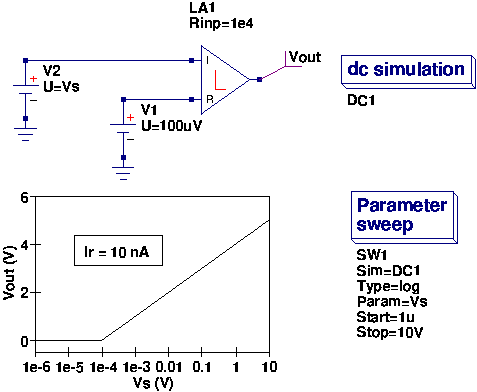
\includegraphics[width=0.6\linewidth]{log_amp_Fig1}
  \caption{Qucs schematic for a basic voltage driven logarithmic amplifier and simulated DC transfer function}
  \label{fig:log_amp1}
\end{figure} 

\begin{figure}
  \centering
  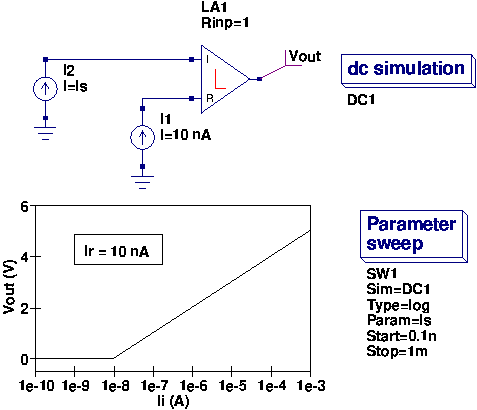
\includegraphics[width=0.6\linewidth]{log_amp_Fig2}
  \caption{Qucs schematic for a basic current driven logarithmic amplifier and simulated DC transfer function}
  \label{fig:log_amp2}
\end{figure} 

\tutsection{Functional description of the Verilog-A logarithmic amplifier macromodel}

The macromodel of a general purpose logarithmic amplifier presented in
previous sections simulates the following device characteristics:
\begin{itemize}
 \item Input stage  : Scaling resistances and DC bias currents.
 \item Gain  stage  : Logarithmic base ten transfer function over $N$ decades with a single pole frequency response. Errors; gain scale and log conformity.
 \item Output stage : Resistance and DC offset voltage.
 \item Properties with temperature variation : gain scale, log conformity, bias currents and output offset voltage.
\end{itemize}

\tutsubsection{Input stage}
The input stage is represented by the Verilog-A code listed in this subsection of the report. The voltages at input terminals $P_{I1}$ and $P_{Ir}$ are divided by scaling resistors $R$ to give the required input currents.  When $R$ is small the input stage operates in current mode. 

\begin{lstlisting}[
 language=Verilog, 
 xleftmargin=12pt,
 basicstyle=\scriptsize]
//
// Input stage
//
I(P_I1) <+ V(P_I1)/R;
I(P_Ir) <+ V(P_Ir)/R;

\end{lstlisting}

\tutsubsection{Gain stage}

The gain stage is represented by the Verilog-A code listed in this
subsection of the report. This part of the model determines the
primary logarithmic amplifier transfer function, including logarithmic
characteristics, frequency response, errors and temperature
effects. An if-else statement is used to test if the log function
argument is greater than one, setting the transfer function output to
zero when the test fails. Both error terms and temperature factors
have been included in the amplifier transfer function
equation. Logarithmic amplifier transfer function frequency response
is normally a complex function of input currents and an internal
frequency compensation capacitance.  Manufacturer's data sheets
usually provide curves of frequency response for typical values of
input current and compensation capacitance. Frequency effects are
represented in the macromodel by a single pole response. The 3dB
corner frequency being set by device parameter $Fc$. The default value
of 3 kHz should be changed to suit the circuit operating conditions.
Figure~\ref{fig:log_amp3} illustrates a small signal test circuit
which allows amplifier transfer function frequency response to be
simulated.

\begin{lstlisting}[
 language=Verilog, 
 xleftmargin=12pt,
 basicstyle=\scriptsize]
//
// Constants
//
PI=3.14159265358979323846;
//
// Model equations
//
V1=V(P_I1);
V2=V(P_Ir)+1e-20;
R=Rinp+1e-6;
Cc=1/(2*PI*Fc);
//
TempK=$temperature;
TnomK=Tnom+273.15;
Tdiff=TempK-TnomK;
NTemp=N+Ntc*Tdiff;
VosoutTemp=Vosout+Vosouttc*Tdiff;
DkTemp=Dk+Dktc*Tdiff;
Ib1Temp=Ib1+Ib1tc*Tdiff;
IbrTemp=Ibr+Ibrtc*Tdiff;
//
if (V1 >= V2 ) Ix = Kv*(1+DkTemp/100)*log(((V1/R)-Ib1Temp)/((V2/R)-IbrTemp))+
                    (Kv*2*(NTemp/100)*M)+VosoutTemp ;
else Ix = 0.0;
..
..
..
//
// Log function stage
//
I(n3) <+ -Ix;
I(n3) <+ V(n3);
//
// Frequency compensation
//
I(n4) <+ -V(n3);
I(n4) <+ V(n4);
I(n4) <+ ddt(Cc*V(n4));
\end{lstlisting}

\begin{figure}
  \centering
  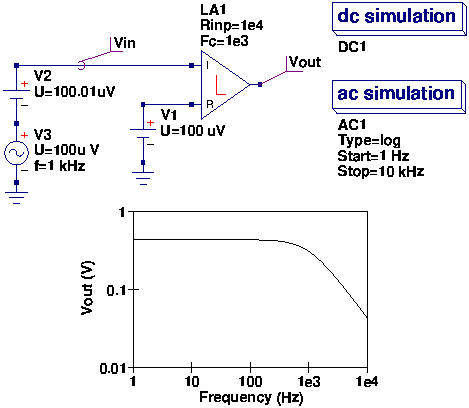
\includegraphics[width=0.6\linewidth]{log_amp_Fig3}
  \caption{Qucs small signal AC test circuit and simulated transfer function}
  \label{fig:log_amp3}
\end{figure} 


\tutsubsection{Output stage}

The output stage is represented by the Verilog-A code listed in this
subsection of the report. This final section of the model introduces
an output resistance $R0$. In a practical logarithmic amplifier this
is often low in value.

\begin{lstlisting}[
 language=Verilog, 
 xleftmargin=12pt,
 basicstyle=\scriptsize]
//
// Output stage
I(P_Vout) <+ -V(n4)/Ro;
I(P_Vout) <+ V(P_Vout)/Ro;
\end{lstlisting}

\tutsection{Logarithmic amplifier large signal AC response} 

The circuit and waveforms presented in Fig.~\ref{fig:log_amp4}
illustrate how the large signal AC response of a logarithmic amplifier
can be tested and displayed. In this circuit a 100 Hz, 1.9 V peak
sinewave signal, in series with a 2V battery, is applied to amplifier
input I. Amplifier reference R has a 0.1V battery connected as the
reference signal. As the logarithmic amplifier output signal is
proportional to the log of the ratio of the input signals $I/R$, the
shape of resulting output signal differs considerably from that of the
excitation sinewave. When the peak of the input sinewave is 1.9 V the
input ratio is 29 and when the negative peak reaches -1.9 V, the ratio
is 1, yielding an output waveform with signal values between log(29)
and 0. This example test circuit once again demonstrates the
compression properties of logarithmic amplifiers.

\begin{figure} [h]
  \centering
  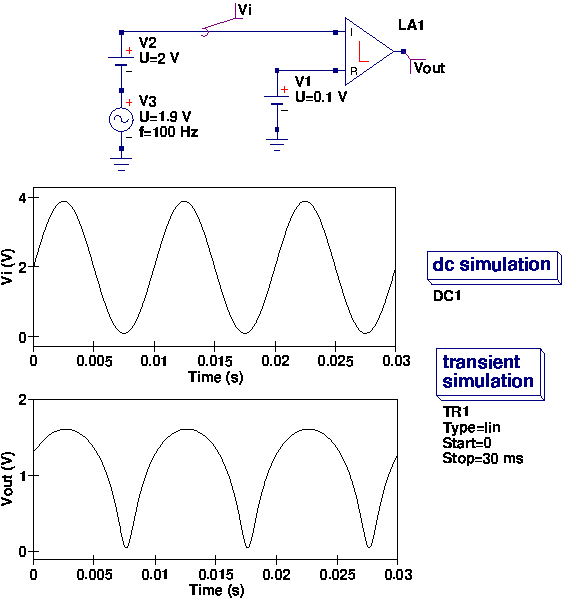
\includegraphics[width=0.6\linewidth]{log_amp_Fig4}
  \caption{Qucs large signal logarithmic amplifier AC test circuit and simulated transient response}
  \label{fig:log_amp4}  
\end{figure} 


\tutsection{Logarithmic amplifier transfer function temperature variation} 

The test circuit shown in Fig.~\ref{fig:log_amp_temp} introduces a
double sweep which changes the amplifier circuit temperature from -110
to 100 Celsius, while simultaneously at each temperature, simulates,
records and displays the amplifier transfer function. In this very
basic example of amplifier response to temperature changes all circuit
dependent parameters are varied at the same time and no attempt is
made to identify individual parameter contributions to the overall
temperature dependency. From the results of this simple test the
simulation waveforms indicate that the typical temperature
coefficients only have minimal effect on circuit performance. Modern
integrated logarithmic amplifies are, in general, well temperature
compensated, minimising the effects of temperature changes on circuit
performance.

\begin{figure} [h]
  \centering
  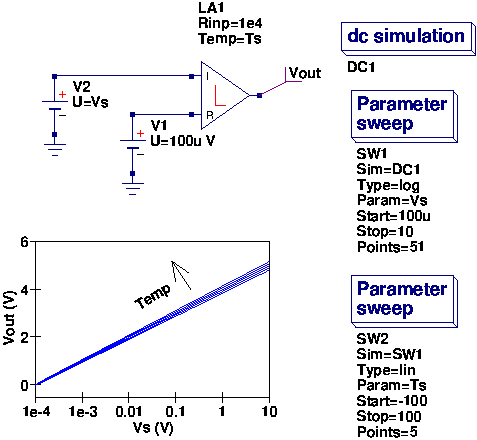
\includegraphics[width=0.6\linewidth]{log_amp_Fig_temp}
  \caption{Qucs logarithmic amplifier transfer function test circuit and simulated temperature response}
  \label{fig:log_amp_temp}
\end{figure} 


\tutsection{Logarithmic amplifier applications}

In this section of this brief report two applications of the
logarithmic amplifier are introduced. These examples are also used to
demonsrate how Verilog-A modelled devices can be merged with other
Qucs built-in components, subcircuits and equation defined
devices. The application examples have been chosen to illustrate the
power of Qucs modelling and simulation.

\tutsubsection{A simple signal multiplier}

One of the most basic, and earliest, applications of the logarithmic
amplifier was signal multiplication. Figure~\ref{fig:log_amp7} shows a
test circuit which includes two logarithmic amplifiers, two voltage
controlled voltages sources (these act as a voltage summer) and an
antilog amplifier.

 \begin{figure} [h]
  \centering
  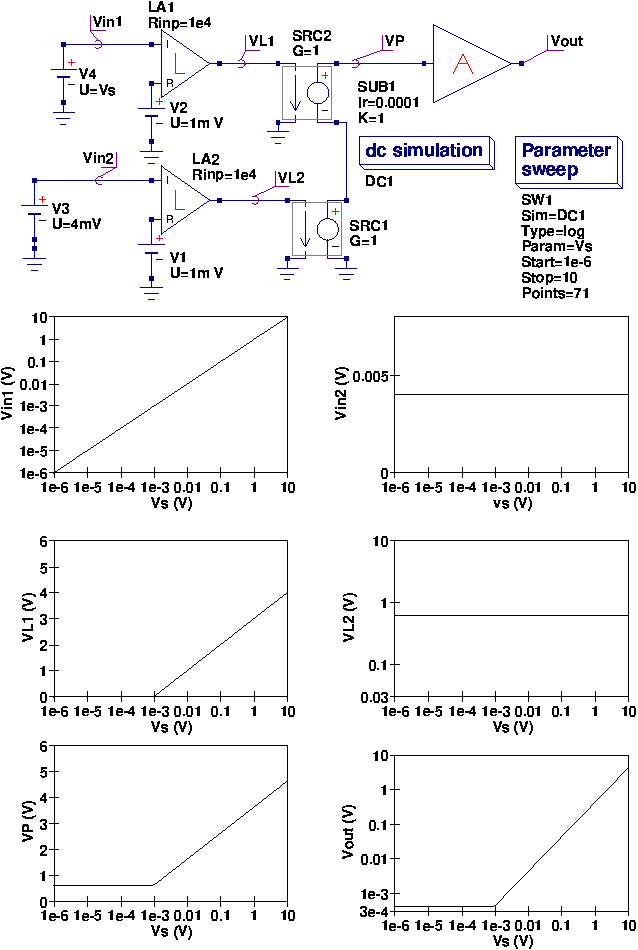
\includegraphics[width=0.55\linewidth]{log_amp_Fig7}
  \caption{A simple electronic multiplier circuit and test waveforms}
  \label{fig:log_amp7}
\end{figure} 
 
The circuit illustrated in Fig.~\ref{fig:log_amp7} multiplies the
ratios of the two sets of inputs.  This is done by taking the log of
each input ratio then adding the results and finally finding the
antilog of the sum. The antilog of a voltage can be found using the
circuit shown in Fig.~\ref{fig:log_ampA}. Parameters Ir and K are used
to scale the output voltage. This must be within the power supply
range of a practical device. In the example shown in
Fig.~\ref{fig:log_amp7} the second input ratio is constant at 4 and
the first has a maximum value of 10/1e-3 = 1e4, causing the output
result to be 4e4 which is way beyond the output voltage of a practical
circuit. By setting k=1 and Ir to 1e-4 the output voltage is scaled so
that the maximum output becomes roughly 4 volts.

 \begin{figure} [h]
  \centering
  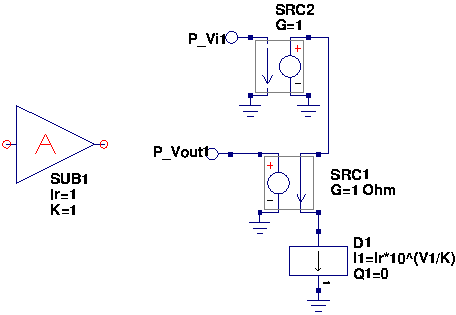
\includegraphics[width=0.55\linewidth]{log_amp_A}
  \caption{A simple antilog amplifier based on a single equation defined device: Controlled source SRC2 acts as a buffer and source SCR1 converts EDD current I1 to voltage}
  \label{fig:log_ampA}
\end{figure} 

\tutsubsection{Light absorption measurements using photodiodes and a log amplifier}

A number of years ago a colleague in Germany made the profound remark
that the 20th century was the century of the electron and that the
21st century was likely to be the century of the photon.  The current
state of Qucs model development does to some extent reflect this
thinking.  At present the major modelling tasks involve extending the
Qucs component/model range and the improvement of their individual
performances. Looking through the current device/model list
immediately confirms that it is dominated by electrical components and
other domain devices, such as transducers, actuators and optical
components, are non-existant. The logarithmic amplifier application
reported here attempts to address this imbalance by providing some
preliminary information on an area of modelling where significant work
is likely to be done in the coming cycles of Qucs development, namely
optical components. Optoelectronic devices, such as LEDs and
photodiodes, are well established in the current electronics
scene. Unfortunately, to my knowledge, Qucs lacks the models for such
devices. The test circuit shown in Fig.~\ref{fig:log_amp9} presents a
basic arrangement for measuring the light absorption properties of
liquids. This is a classical application of the logarithmic amplifier,
working as a device that measures the ratio of two currents. These
currents are generated by photodiodes.

In Fig.~\ref{fig:log_amp9} a light source shines on two photodiodes:
directly on one and indirectly on the other. In the second case the
light travels through a vessel containing a liquid which attenuates
the light. The level of attenuation being dependent on the light
absorption properties of the liquid.  When little or no light is
absorbed the logarithmic amplifier output is small. However, at high
light absorption levels the amplifier output is high. The circuit
given in Fig.~\ref{fig:log_amp9} works over six decades of light
transmission coefficient. Moreover, it does not require the absolute
values of the light intensities to be measured. The circuit output
voltage is compressed to a range between 0 and 5 volts which is ideal
for interfacing with a unipolar analogue-to-digital converter. Qucs
cannot represent light signals directly. However, it is possible to
use a voltage to represent the intensity of a light. Once one realises
that the numerical value of light intensity can be represented by a
voltage of the same numerical value then it also becomes possible to
represent light signals paths by nets with specific voltage values.
In Fig.~\ref{fig:log_amp9} the light paths are represented by wires
connecting the light source, the liquid vessel and the
photodiodes. Models for the light absorbing liquid and the photodiodes
are shown in Fig.~\ref{fig:log_amp10}.


 \begin{figure} [h]
  \centering
  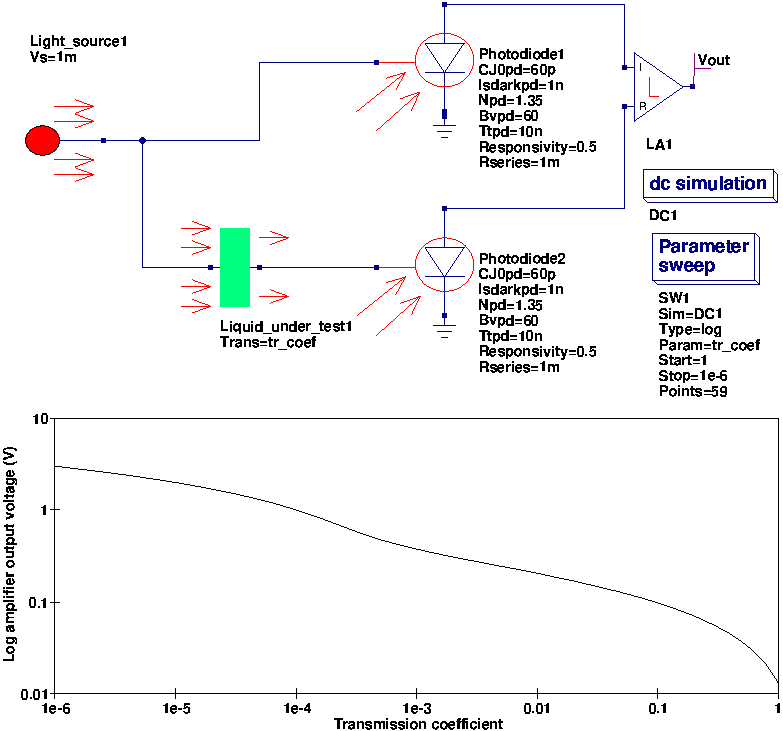
\includegraphics[width=0.9\linewidth]{log_amp_Fig9}
  \caption{Light absorption measurements using photodiodes and a logarithmic amplifier}
  \label{fig:log_amp9}
\end{figure}   


 \begin{figure} [h]
  \centering
  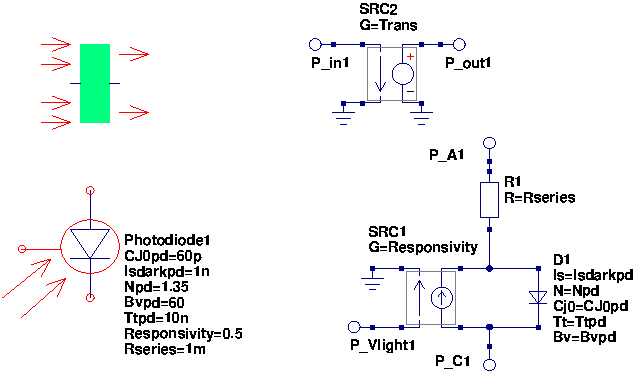
\includegraphics[width=0.9\linewidth]{log_amp_Fig10}
  \caption{Experimental Qucs models for a light absorbing liquid and a photodiode}
  \label{fig:log_amp10}
\end{figure}

In Fig.~\ref{fig:log_amp10} the light absorbing liquid is represented
by a voltage controlled voltage source where the source gain models
the transmission coefficient: a gain of one implies 100\verb|%|
transmission and a gain of zero no light transmission at all. The
photodiode model is much more complex.  A voltage controlled current
source in parallel with a diode forms the core of the model.  The gain
of the controlled source represents the responsivity of the
diode. Responsivity is expressed in amperes per watt or as the
photodiode current for a given input light power per unit area. As the
current generated is also expressed as the current per unit area,
effectively the area factor is eliminated.  Equation \eqref{eq:id}
relates the photodiode current to the voltage at the light input
terminal:
\begin{equation}
\label{eq:id}
Id=Responsivity\cdot V(PVlight)
\end{equation}

Responsivity is a function of the light wavelength and is around 0.5
to 0.6 for wavelengths of 900nm. It is roughly 0.3 for blue
wavelengths and drops to 0.2 in the ultraviolet region of the
spectrum. With no illumination falling on a photodiode the resulting
diode current is small, being called the device dark current. It
ranges from tens of pA for ultraviolet detecting photodiodes to
several $\mu A$ for low cost silicon diodes. Typical values for
Rseries are in the range 1m to 20m$\Omega$.  The other parameters are
similar to those representing standard semiconductor diodes but with
values specifically chosen to represent the properties of photodiodes.

\tutsection{End note}

These notes summarise a basic technique for modelling logarithmic
amplifiers using Verilog-A.  Verilog-A is primarily intended for
modelling compact semiconductor devices.  However, as this report
demonstrates it can be equally employed for macromodelling of
integrated circuits and circuits in general. The Qucs C++ code for the
modular operational amplifier model, generated by ADMS, can be found
in the Qucs release archives at
\url{http://qucs.sourceforge.net/download.html}.  The procedure
undertaken to convert the Verilog-A code into C++ for compilation and
linking with Qucs closely followed that described by Stefan Jahn and
H\'{e}l\`{e}ne Parruitte.  Although it takes more work to construct
models using ADMS the effort is worthwile because the finished models
are very efficient in terms of memory usage and have significantly
reduced run times. It is worth noting that Verilog-A based models can
be combined with other forms of Qucs model, forming a powerful
combination that extends Qucs simulation capabilities. Once again a
special thanks to Stefan Jahn for all his help and encouragement over
the period that I have been developing the Verilog-A logarithmic
amplifier macromodel, writing this report and testing the examples it
includes.
